\documentclass[12pt, a4paper]{article}

\usepackage[utf8]{inputenc}
\usepackage[T1]{fontenc}
\usepackage[spanish,es-noquoting]{babel}

% Secciones
\usepackage{titlesec}
\newcommand{\sectionbreak}{\clearpage}

% Matemáticas
\usepackage{amsmath, amssymb, amsthm}
\usepackage{mathtools}
\usepackage{bm}

% Diseño de página
\usepackage[top=2.5cm, bottom=2.5cm, left=3cm, right=2.5cm]{geometry}
\usepackage{setspace}
\onehalfspacing

% Figuras y tablas
\usepackage{graphicx}
\usepackage{float}
\usepackage{booktabs}
\usepackage{array}
\usepackage{multirow}
\usepackage{longtable}
\usepackage{caption}
\usepackage{subcaption}

% Cabeceras
\usepackage{fancyhdr}
\pagestyle{fancy}
\fancyhf{}
\fancyhead[L]{\small Computación Concurrente}
\fancyhead[R]{\small Introducción al Cómputo Concurrente}
\fancyfoot[C]{\thepage}
\renewcommand{\headrulewidth}{0.4pt}

\begin{document}

\begin{titlepage}
    \centering
    {\bfseries\LARGE Universidad Nacional Autónoma de México \par}
    \vspace{0.5cm}
    {\scshape\Large Facultad de Ciencias \par}
    \vspace{0.5cm}
    {\bfseries\large Ciencias de la Computación \par}
    \vspace{1cm}
    
    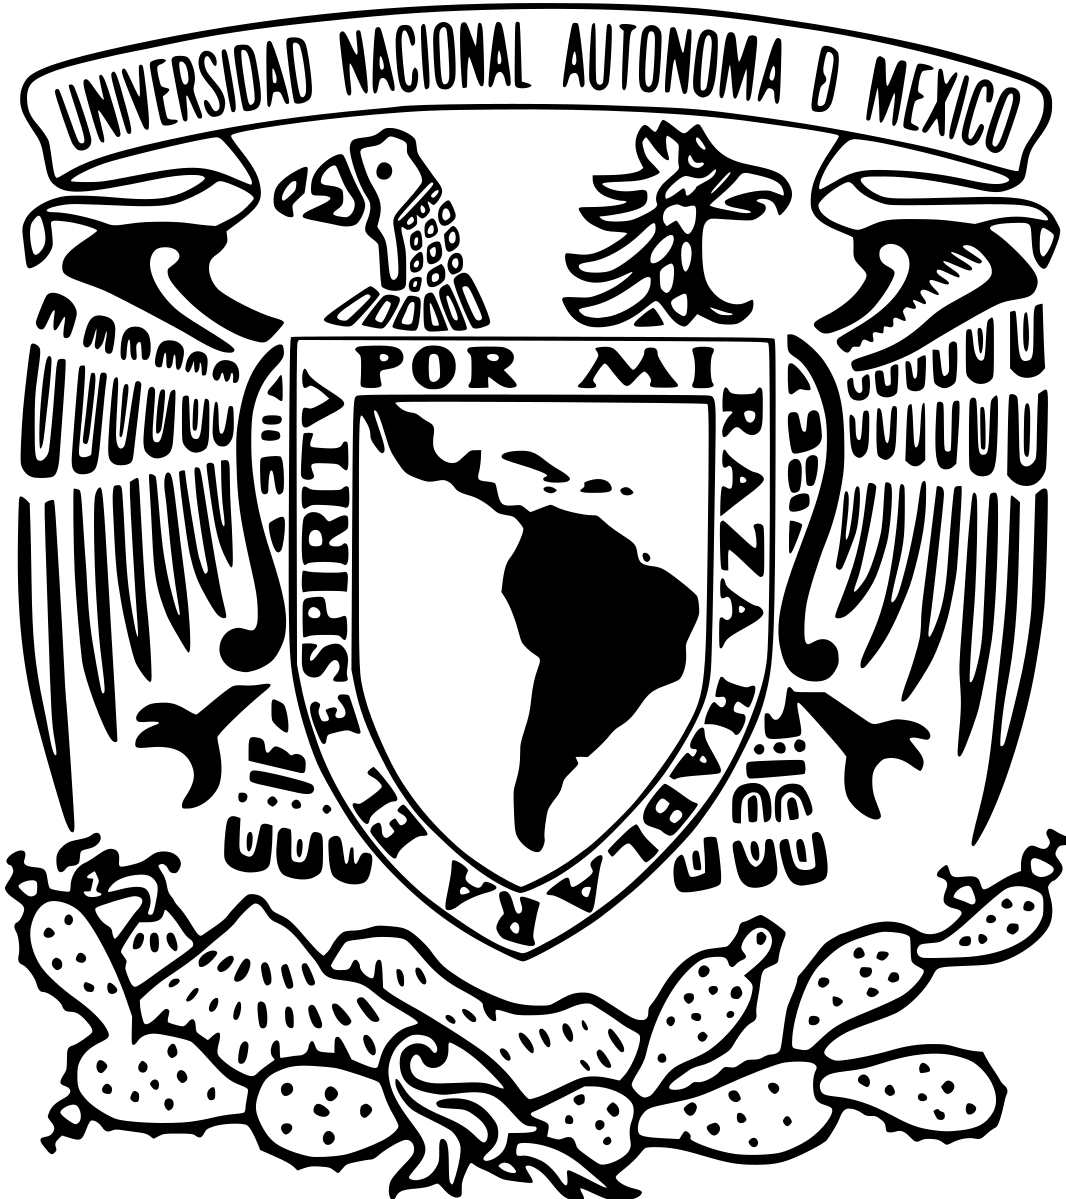
\includegraphics[width=0.3\textwidth]{imgs/unam_logo.png}\par
    \vspace{1cm}

    {\Large Criptografía y Seguridad}
    \vspace{1cm}

    \rule{\linewidth}{0.5mm}\\[0.4cm]
    {\Huge\bfseries Práctica 1\par}
    \vspace{0.5cm}
    {\Large\bfseries Cifrados Clásicos \par}
    \vspace{0.5cm}
    \rule{\linewidth}{0.5mm}\\[0.4cm]
    
    {\Large Aguirre Cruz Cassandra - \par}
    {\Large González Téllez Lorena - 321288952 \par}
    {\Large Vázquez Rincón Oscar -  321228954\par}
    
    \vfill
    
    {\large \today \par}
    
\end{titlepage}

% -------------------------------------------------------------------------------------------------------------------

\section{Introducción}

La criptografía es la ciencia encargada de diseñar funciones o dispositivos capaces de transformar mensajes legibles
o en claro a mensajes cifrados de tal manera que dicha transformación (cifrar) y su transformación inversa (descifrar)
sólo pueden ser factibles con el conocimiento de una o más llaves. En la criptografía existen dos tipos de cifrados: los simétricos, en donde la misma llave se usa para cifrar y descifrar, y los asimétricos, 
en donde se utilizan dos llaves distintas. Esta práctica se centra en los cifrados simétricos.

Los cifrados clásicos son aquellos que han tenido un uso histórico masivo, pero que hoy en día no se consideran
seguros, pues han surgido técnicas modernas más sofisticadas a lo largo del tiempo.

Esta práctica tiene como objetivo implementar algunos de estos cifrados clásicos y aplicarlos para el cifrado y el
descifrado de archivos. El desarrollo de la misma implica trabajar directamente a nivel de bytes y realizar corrimientos correspondientes según el cifrado empleado. El enfoque se centra en el cifrado César, el cifrado
decimado, el cifrado afín y la codificación Base64. Para poder descifrar los archivos sin conocer
la llave de antemano, se hace uso de las firmas de archivo o Magic Bytes. Se busca combinar este conocimiento con las propiedades 
matemáticas de los cifrados para deducir la llave correcta y recuperar los archivos originales.

La importancia de esta práctica radica en comprender la base y los cimientos de lo que es la
criptografía moderna. Saber aplicar estos cifrados clásicos permite construir bases sólidas sobre el origen de la disciplina,
aplicando congruencias y aritmética modular. Por otro lado, el enfrentarse a un escenario de descifrado, como el que plantea 
esta práctica, nos permite desarrollar conocimientos sobre el manejo de bytes y las firmas de archivo.

% -------------------------------------------------------------------------------------------------------------------

\section{Desarrollo}

El desarrollo de esta práctica consta de distintas etapas: los cifrados, las firmas de los archivos y el manejo de bytes.

\subsection{Cifrados}

Los cifrados implementados en esta práctica se encuentran en el archivo \texttt{cifrados\_clasicos.py}.
A continuación se describe el procedimiento de desarrollo de cada uno.

\subsubsection*{Cifrado César}

El cifrado César es un cifrado de sustitución. De acuerdo a [Notas Galaviz], si en un mensaje original se
encuentra el símbolo de índice $i$ de un alfabeto de $n$ símbolos y al cifrarlo se le substituye por el símbolo
de índice $j$ del alfabeto desplazado de $k$ lugares a la derecha, entonces podemos simbolizar el cifrado como:

\[
    j \equiv (i + k) \pmod n
\]

Dado que en esta práctica haremos el manejo de arhivos a nivel de bytes, el alfabeto que usaremos está compuesto 
por los valores de los bytes, es decir, $n = 256$ y los caracteres son los valores enteros en el rango $[0, 255]$. 
La llave $k$ es un entero en el rango $[0, 255]$.

\begin{itemize}

    \item \textbf{Cifrado:} La función \texttt{cesar\_cifrar(data, k)} recibe la secuencia de bytes \texttt{data}
y la llave entera $k$. Se itera sobre todos los bytes del mensaje (de acuerdo a la definición anterior) y se construye 
el resultado como un objeto \texttt{bytes}:

\begin{verbatim}
resultado = bytes((byte + k) % 256 for byte in data)
\end{verbatim}

    \item \textbf{Descifrado:} La función \texttt{cesar\_descifrar(data, k)} aplica lo inverso del cifrado y para ello
    se resta $k$ a cada byte del mensaje (regresando el mismo número de lugares que se avanzó en el cifrado). 
    De manera análoga la implementación es:

\begin{verbatim}
resultado = bytes((byte - k) % 256 for byte in data)
\end{verbatim}

\end{itemize}

\subsubsection*{Inverso modular}

Como parte de los cifrados Decimado y Afín es necesario calcular el
inverso modular de la llave $a \in \mathbb{Z}_{256}$ respecto del módulo 256.
El inverso modular $x$ de $a$ módulo $m$ es el entero que satisface:

\[
    (a \cdot x) \equiv 1 \pmod m
\]

La función \texttt{inverso\_modular(a, m)} se calcula mediante el
algoritmo de Euclides extendido:

\begin{verbatim}
m_original = m
x0 = 1
x1 = 0
while m != 0:
    cociente = a // m
    a, m = m, a % m
    x0, x1 = x1, x0 - cociente * x1
if a != 1:
    raise ValueError("Si no existe el inverso modular")
return x0 % m_original
\end{verbatim}

A continuación veremos que su uso es imperativo en los otros cifrados.

\subsubsection*{Cifrado Decimado}

Este esquema es similar al cifrado César, pero ahora el símbolo que reemplaza al $i$-ésimo es obtenido
multiplicando $i$ por algún número, es decir, el $i$-ésimo símbolo es reemplazado en el texto cifrado por
el $j$-ésimo con $j = (ki) \bmod n$. Para que el cifrado sea válido en nuestros bytes y cumpla con ser 
una función biyectiva, es necesario elegir el factor de decimación de modo que sea primo relativo a $n = 256$.

\begin{itemize}
    \item \textbf{Cifrado:} La función \texttt{decimado\_cifrar(data, a)} multiplica cada byte
    del mensaje por la llave $a$ y reduce módulo 256. La lógica es la siguiente:
\begin{enumerate}
    \item Realizamos $a \bmod 256$ para que la llave esté en el rango $[0, 255]$.
    \item Verificamos que $\gcd(a, 256) = 1$ llamando a \texttt{inverso\_modular(a, 256)}. Esto nos 
            asegura de que la transformación sea biyectiva. De no cumplirse, no sería válido el cifrado
            porque no nos asegura que la función de cifrado sea biyectiva y por tanto el descifrado no
            sería posible.
    \item Aplicamos la transformación de multiplicación byte a byte.
\end{enumerate}

\begin{verbatim}
a = a % 256
inverso_modular(a, 256)
resultado = bytes((byte * a) % 256 for byte in data)
\end{verbatim}

    \item \textbf{Descifrado:} La función \texttt{decimado\_descifrar(data, a)} invierte el cifrado. Contrario
    al cifrado César, se multiplica por el inverso modular de $a$ módulo 256 para recuperar el mensaje original.
    La lógica implementada es:
    \begin{enumerate}
        \item Aplicamos $a \pmod {256}$ para que esté en el rango $[0, 255]$.
        \item Calculamos el inverso modular de $a$ mediante \texttt{inverso\_modular(a, 256)}.
        \item Aplicamos la transformación de multiplicación inversa byte a byte.
    \end{enumerate}

\begin{verbatim}
a = a % 256
inverso = inverso_modular(a, 256)
resultado = bytes((byte * inverso) % 256 for byte in data)
\end{verbatim}


\end{itemize}

\textbf{Observación:} Para que el cifrado sea reversible, $a$ debe ser coprimo con 256, es decir,
$\gcd(a, 256) = 1$. En el programa se define \texttt{LLAVES} como el conjunto de llaves válidas. En el 
intervalo $[1, 255]$ hay exactamente $\phi(256) = 128$ valores válidos.

\subsubsection*{Cifrado Afín}

Este cifrado consiste de una combinación de los dos cifrados anteriores donde la regla de sustitución está dada por
$j = (ri + k) \pmod n$, donde $i,r,k \in \{0, \dots, n-1\}$. Recordando que para nuestro caso $n=256$: $i,r,k \in \{0, \dots, 255\}$. 
Igual que en el cifrado Decimado, también necesitamos que la transformación sea biyectiva, y por tanto, $r$ debe ser coprimo con $n=256$.

\begin{itemize}
    \item \textbf{Cifrado:} La función \texttt{afin\_cifrar(data, a, b)} aplica a cada byte la transformación que
    acabamos de mencionar. La lógica se sigue de:

\begin{enumerate}
    \item Nos aseguramos que las llaves estén en $\{0,  \cdots, 255\}$: $a \bmod 256$, $b \bmod 256$.
    \item Verificamos que $\gcd(a, 256) = 1$ para que la función de cifrado sea biyectiva.
    \item Aplicamos la transformación definida byte a byte.
\end{enumerate}

\begin{verbatim}
a = a % 256
b = b % 256
inverso_modular(a, 256)
resultado = bytes((a * byte + b) % 256 for byte in data)
\end{verbatim}
    
    \item \textbf{Descifrado:} La función \texttt{afin\_descifrar(data, a, b)} invierte la transformación afín.
Considerando que en el cifrado $j = (a \cdot i + b) \bmod 256$ se despeja $i$ que es el dato original que queremos
recuperar mediante la siguiente expresión:

\[
    i = (a^{-1} \cdot (j - b)) \bmod 256
\]

De modo que la lógica de descifrado está dada por:
\begin{enumerate}
    \item Obtenemos los valores de las llaves $a \bmod 256$ y $b \bmod 256$.
    \item Calculamos el inverso modular $a^{-1}$ de $a$ módulo 256.
    \item Aplicamos la transformación inversa byte a byte.
\end{enumerate}

\begin{verbatim}
a = a % 256
b = b % 256
inverso = inverso_modular(a, 256)
resultado = bytes((inverso * (byte - b)) % 256 for byte in data)
\end{verbatim}
\end{itemize}

\subsubsection*{Base64}

En esta codificación se convierte la secuencia de bytes en una secuencia de caracteres (en este caso ASCII),
fue implementada en el archivo \texttt{base64.py}. La idea es que tres valores de byte de datos se codifican en
cuatro valores Base64.

Primero es importante mencionar que el alfabeto de 64 caracteres se definió por el alfabeto:

\begin{verbatim}
CARACTERES = "ABCDEFGHIJKLMNOPQRSTUVWXYZabcdefghijklmnopqrstuvwxyz0123456789+/"
\end{verbatim}

Cada posición $i \in [0, 63]$ corresponde a un bloque de 6 bits con valor $i$.

\begin{itemize}
    \item \textbf{Codificación:} La función \texttt{base64\_encode} recibe una cadena binaria y aplica el siguiente
    procedimiento:

    \begin{enumerate}
        \item Determinar cuántos bytes completos de 3 caracteres forman la entrada. Determinando si la longitud es o no
        múltiplo de $3$, se calcula cuántos caracteres de relleno son necesarios.

\begin{verbatim}
completo = len(data) % 3
p = 0 if completo == 0 else (3 - completo)
\end{verbatim}

    \item Se rellena hasta que la longitud sea múltiplo de 3, y luego cada byte se convierte a su representación 
    binaria.
    
\begin{verbatim}
data_padded = data + b"\x00" * p
bits = "".join(format(b, "08b") for b in data_padded)
\end{verbatim}

    \item Recorremos la cadena binaria en bloques de 6 bits y se transforman a enteros en base 2 (como índices) 
    para obtener el caracter correspondiente Base64 usando el alfabeto ya mencionado.

\begin{verbatim}
res = "".join(CARACTERES[int(data[i:i+6], 2)]
              for i in range(0, len(data), 6))
\end{verbatim}

    \item Finalmente, si $p > 0$, sustituimos los últimos $p$ caracteres por \texttt{'='}.

\begin{verbatim}
if p > 0:
    res = res[:-p] + ("=" * p)
\end{verbatim}

    \end{enumerate}


    \item \textbf{Decodificación:} Para poder decodificar el procedimiento anterior, se implementó la función
    \texttt{base64\_decode} que recibe la cadena obtenida en Base64 y realiza el siguiente procedimiento para 
    recuperar los bytes:

    \begin{enumerate}
    \item Mediante un diccionario se asocia cada caracter del alfabeto el índice numérico de 6 bits.

\begin{verbatim}
BUSQUEDA = {c: i for i, c in enumerate(CARACTERES)}
\end{verbatim}

    \item Se eliminan los caracteres de relleno '=' de la cadena.

\begin{verbatim}
padding = encoded.count("=")
word = encoded.replace("=", "")
\end{verbatim}

    \item Se transforman los caracteres a los índices correspondientes.

\begin{verbatim}
vals = [BUSQUEDA[c] for c in word if c in BUSQUEDA]
\end{verbatim}

    \item Se transforma a múltiplos de 4 rellenando con ceros, esto porque cada 4 bloques de 6 bits forman
    exactamente $4 \times 6 = 24$ bits (3 bytes).

\begin{verbatim}
while len(vals) % 4 != 0:
    vals.append(0)
\end{verbatim}

    \item Con desplazamientos bit a bit, por cada bloque de 4 valores se une unn entero de 24 bits,
    lo que nos permite formar los 3 bytes que lo formaron desde un inicio:

\begin{verbatim}
result = bytearray()
for i in range(0, len(vals), 4):
    n = (vals[i] << 18) | (vals[i+1] << 12) | (vals[i+2] << 6) | vals[i+3]
    result.append((n >> 16) & 0xFF)
    result.append((n >> 8) & 0xFF)
    result.append(n & 0xFF)
\end{verbatim}

    \item Se eliminan los bytes de relleno que habíamos añadido en la codificación.

\begin{verbatim}
if padding:
    del result[-padding:]
\end{verbatim}

    \end{enumerate}
\end{itemize}


\subsection{Firmas de Archivos}

Para esta etapa de la práctica se implementó el archivo \texttt{magic\_bytes.py},
cuyo propósito es identificar el formato real de un archivo a partir de su
contenido binario. Dado que las extensiones de los archivos pueden ser alteradas, 
los formatos binarios incluyen al inicio del archivo una secuencia fija de bytes 
que permite identificar el formato.

Como parte de la implementación se definió el diccionario \texttt{MAGIC\_BYTES\_HEX} 
que mapea la representación hexadecimal de cada firma al nombre de su formato:

\begin{verbatim}
MAGIC_BYTES_HEX = {
    "89504e470d0a1a0a": "png",
    "ffd8ff":           "jpg",
    "424d":             "bmp",
    "494433":           "mp3",
    "fffb":             "mp3",
    "4f676753":         "ogg",
    "0000001866747970": "mp4",
    "1a45dfa3":         "mkv",
    "504b0304":         "docx",
    "25504446":         "pdf",
    "65707562":         "epub",
}
RIFF = "52494646"
\end{verbatim}

Además, se definió la constante \texttt{RIFF = "52494646"} para manejar
de forma especial los formatos WAV y AVI, que comparten los mismos 4 bytes
iniciales \texttt{52 49 46 46}.

La función \texttt{detectar\_formato(data)} recibe el contenido binario de un
archivo y determina su formato. El procedimiento es el siguiente:

\begin{enumerate}
    \item Se extraen los primeros 16 bytes del archivo, tanto para flujos
          de datos (objetos con método \texttt{read}) como para secuencias de bytes:

\begin{verbatim}
if hasattr(data, 'read'):
    start_pos = data.tell() if hasattr(data, 'tell') else 0
    bytes_data = data.read(16)
    if hasattr(data, 'seek'):
        data.seek(start_pos)
else:
    bytes_data = data[:16]
\end{verbatim}

    \item Los bytes extraídos se convierten a su representación hexadecimal en minúsculas:

\begin{verbatim}
hexbytes = bytes_data.hex()
\end{verbatim}

    \item Si los primeros 4 bytes corresponden a RIFF (\texttt{52494646}), no es posible
          distinguir WAV de AVI y se inspeccionan los bytes 8 a 11 del archivo. Si no coinciden con alguno, 
          devuelve \texttt{None}:

\begin{verbatim}
if hexbytes.startswith(RIFF) and len(bytes_data) >= 12:
    subtype = bytes_data[8:12]
    if subtype == b"WAVE": return "wav"
    if subtype == b"AVI ": return "avi"
    return None
\end{verbatim}

    \item Se itera sobre el diccionario \texttt{MAGIC\_BYTES\_HEX}. Al encontrar una
          coincidencia devuelve el formato correspondiente:

\begin{verbatim}
for magic_hex, formato in MAGIC_BYTES_HEX.items():
    if hexbytes.startswith(magic_hex):
        return formato
return None
\end{verbatim}

    \item Si ninguna firma coincide, la función retorna \texttt{None}.
\end{enumerate}

\subsection{Manipulación de bytes}

El archivo \texttt{archivos\_bytes.py} fue implementado para manejar las operaciones
de entrada a nivel de bytes.

La función \texttt{leer\_archivo(ruta)} recibe la ruta de un archivo y devuelve su contenido 
completo como un objeto \texttt{bytes}. Para ello comprueba que que el archivo existe en la ruta
recibida y luego se abre el archivo en modo binario.

El uso del modo binario es necesario ya que los cifrados
operan directamente sobre los valores numéricos de cada byte (0--255).

\subsection{Descifrador de Archivos}

Después de todas las implementaciones anteriores se implementó el programa \texttt{main.py} que
integra el proceso de descifrado de un archivo del cual no conocemos su cifrado ni sus llaves. 
Por lo que para poder descifrarlo se aplicó fuerza bruta probando algoritmo por algoritmo con 
todas las posibles llaves, esto hasta encontrar el correcto si es que fue cifrado con alguno de los
que implementamos.

Para mantener el código organizado se definieron dos funciones auxiliares:

\begin{itemize}
    \item \texttt{guardar(datos, nombre\_base, formato)}: Para guardar los archivos que se descifren correctamente.
    \item \texttt{resultado(cifrado, llave, formato, ruta)}: Para imprimir un resumen del descifrado.
\end{itemize}

Como mencionamos antes, aplicamos fuerza bruta para cada cifrado. Para hacerlo más efectivo, en cada intento
se opera sobre los primeros 16 bytes para verificar las firmas antes de descifrar el archivo completo. De esta manera,
tenemos una función de fuerza bruta por cada cifrado, en todas estas funciones se intenta descifrar los primeros
16 bytes y si coincide con alguna firma, se descifra el archivo completo (se guarda). Lo que cambia entre ellas es el espacio de 
llaves. Por lo que estas funciones son:

\begin{itemize}
    \item \textbf{Base64} \texttt{base64\_fuerza\_bruta}: Interpreta los bytes como texto ASCII y los decodifica,
    no hay llaves para iterar.

    \item \textbf{César} \texttt{cesar\_fuerza\_bruta}: Itera sobre todas las posibles llaves $k \in \{0, 1, \dots, 255\}$.

    \item \textbf{Decimado} \texttt{decimado\_fuerza\_bruta}: Itera sobre todas las llaves coprimas con 256.

    \item \textbf{Afín} \texttt{afin\_fuerza\_bruta}: Itera sobre todas las posibles llaves $(a, c)$ con
    \texttt{a} coprimo con 256.
\end{itemize}

Como resultado final, la función \texttt{descifrar\_archivo(ruta\_cifrado)} une toda la lógica de descifrado
que hemos ido desarrollando:

\begin{enumerate}
    \item Verificar que la ruta recibida corresponde a un archivo existente.
          Si no existe, terminar con error.
    \item Leer el contenido binario completo con \texttt{leer\_archivo}.
    \item Iterar sobre la lista de métodos en orden:
\begin{verbatim}
METODOS_CIFRADO = [
    base64_fuerza_bruta,
    cesar_fuerza_bruta,
    decimado_fuerza_bruta,
    afin_fuerza_bruta,
]
for metodo in METODOS_CIFRADO:
    if metodo(datos, nombre_base):
        break
\end{verbatim}
    \item El primer método que retorne \texttt{True} detiene la búsqueda. De otro modo, se concluye que 
          el archivo no fue cifrado con ninguno de los métodos implementados.
\end{enumerate}

El programa se ejecuta desde la terminal de la siguiente forma:

\begin{verbatim}
python src/main.py <ruta_del_archivo_cifrado>
\end{verbatim}

% -------------------------------------------------------------------------------------------------------------------

\subsection{Preguntas}

\begin{enumerate}

    \item ¿Cuántos primos relativos hay en $\mathbb{Z}_{256}$?

Primero conviene recordar que dos enteros $a, b \in \mathbb{Z}$ son primos relativos si su máximo común divisor
es 1, es decir, si $\gcd(a,b) = 1$.

Por otro lado, $\mathbb{Z}_m$ denota al conjunto de todas las clases de equivalencia diferentes módulo $m$. Donde
cada clase de equivalencia se define como $[z]_m = \{x \in \mathbb{Z} \mid z \equiv x \pmod{m}\}$. De este modo, cuando
hablamos de $\mathbb{Z}_{256}$ nos referimos a un conjunto con $256$ elementos, es decir:
\[
\mathbb{Z}_{256} = \{[0]_{256}, [1]_{256}, [2]_{256}, \dots, [255]_{256}\}
\]

Después de estos recordatorios, para poder contar los primos relativos en $\mathbb{Z}_{256}$ podemos usar la
función indicatriz de Euler. Si $n \in \mathbb{N}$, entonces $\phi(n)$ se define como el número de enteros
positivos menores o iguales a $n$ y coprimos con $n$, es decir, formalmente se puede definir como:

\[
\phi(n) = |\{m \in \mathbb{N} \mid 1 \le m \le n \land \gcd(m, n) = 1\}|
\]

Dentro de las propiedades que nos ofrece la función indicatriz de Euler encontramos que:

\[
\phi(p^k) = (p-1)p^{k-1}\ \text{si } p \text{ es un número primo y } k \in \mathbb{N}
\]

Dado que queremos contar los primos relativos en $\mathbb{Z}_{256}$, conviene ver que $256 = 2^8$. Por lo que $p=2$ 
(pues $2$ es primo) y $k=8 \in \mathbb{N}$ en la propiedad que acabamos de enunciar. Aplicando la fórmula:

\[
\phi(2^8) = (2-1)2^{8-1} = 1 \cdot 2^7 = 128
\]

Esto nos muestra que existen 128 primos relativos en $\mathbb{Z}_{256}$.




    \item Sea $f:\mathbb{Z}_{n}\rightarrow\mathbb{Z}_{n}$ tal que $f(i)=k \cdot i$ para $i\in A$ con $A$ un alfabeto cualquiera. ¿Qué se debe cumplir para que $f$ sea una función biyectiva?

Por definición, para que $f$ sea biyectiva debe cumplirse que sea inyectiva y sobreyectiva al mismo tiempo.

\textbf{Inyectividad:} Para que $f$ sea inyectiva debe cumplirse que no hay dos elementos del dominio
que tengan la misma imagen, es decir, para $a,b \in \mathbb{Z}_n$, si $f(a) = f(b)$, entonces $a=b$.

Supongamos primero que para $a,b \in \mathbb{Z}_n$, $f(a)=f(b)$, es decir, $[k \cdot a]_n = [k \cdot b]_n$.
Recordando que dos clases de equivalencia son iguales si y sólo si sus representantes son congruentes
módulo $n$ ($[x]_n = [y]_n \iff x \equiv y \pmod{n}$) tenemos que $ka \equiv kb \pmod{n}$, lo cual
es equivalente a:
\[
k(a - b) \equiv 0 \pmod{n}
\]
es decir, $n \mid k(a-b)$ (por definición de congruencia). Aquí es importante mencionar que buscamos cancelar el 
factor $k$ para que se cumpla que $n \mid (a-b)$, que por definición de congruencia implicaría $a \equiv b \pmod{n}$.

Para este propósito, recurrimos al Lema de Euclides donde si $n \mid k \cdot m$ y $\gcd(k,n)=1$, entonces $n \mid m$.

De esta manera, si se cumple que $\gcd(k,n)=1$, podemos concluir que $n \mid (a-b)$, es decir, $a \equiv b \pmod{n}$, 
lo que en $\mathbb{Z}_n$ significa que $[a]_n = [b]_n$, por lo tanto $a = b$ y $f$ es inyectiva.

\textbf{Observación:} La condición $\gcd(k,n)=1$ es la hipótesis que necesitamos para que el argumento sea válido.
Si en cambio $\gcd(k, n) = d > 1$, entonces existe $m = n/d$ con $0 < m < n$ tal que $k \cdot m \equiv 0 \pmod{n}$.
Esto se debe a que $d \mid k$ (pues $d = \gcd(k,n)$), por lo que $k = d \cdot q$ para algún $q \in \mathbb{Z}$, y entonces
$k \cdot m = d \cdot q \cdot (n/d) = q \cdot n$, que es claramente múltiplo de $n$. Esto implica $f(m) = [k \cdot m]_n = [0]_n = f(0)$
con $m \neq 0$, por lo que $f$ no sería inyectiva y, por tanto, no sería biyectiva.

\textbf{Sobreyectividad:} Para que $f$ sea sobreyectiva debe cumplirse que todo elemento del codominio
$\mathbb{Z}_n$ es imagen de algún elemento del dominio, es decir, para todo $j \in \mathbb{Z}_n$
existe $i \in \mathbb{Z}_n$ tal que $f(i) = j$.

Ahora bien, si $\gcd(k, n) = 1$, entonces $k$ es invertible en $\mathbb{Z}_n$, es decir, existe
$k^{-1} \in \mathbb{Z}_n$ tal que $k \cdot k^{-1} \equiv 1 \pmod{n}$. Dado un elemento cualquiera
$j \in \mathbb{Z}_n$, basta tomar $i = k^{-1} \cdot j \in \mathbb{Z}_n$, pues:
\[
f(i) = k \cdot (k^{-1} \cdot j) = (k \cdot k^{-1}) \cdot j \equiv 1 \cdot j \equiv j \pmod{n}
\]
Así, todo elemento de $\mathbb{Z}_n$ tiene preimagen y $f$ es sobreyectiva.

$\therefore$ La condición necesaria y suficiente para que $f(i)=k \cdot i$ sea una función
biyectiva en $\mathbb{Z}_n$ es que $\gcd(k, n) = 1$, es decir, que $k$ y $n$ sean primos relativos.


    \item ¿Cuántas posibles combinaciones no triviales existen para cifrar bytes con César, Decimado y Afín?
    \begin{itemize}
        \item \textbf{César:} 255 combinaciones no triviales (256 en total, menos la clave trivial $k=0$).
        \item \textbf{Decimado:} 127 combinaciones no triviales (128 números impares coprimos con 256, menos la clave trivial $a=1$).
        \item \textbf{Afín:} 32,767 combinaciones no triviales ($128 \times 256 = 32,768$ en total, menos la clave trivial $a=1, b=0$).
    \end{itemize}
    \item ¿Por qué el sistema de archivos de UNIX, aunque un archivo tenga una extensión diferente (o incluso no tenga), sigue reconociendo al archivo original?
    \begin{itemize}
    \item UNIX inspecciona el interior del archivo usando los primeros bytes para leer su firma digital, la cual indica el tipo de archivo real. Tambien los metadatos y datos físicos residen todavia. 
    El nombre del archivo y su extensión son solo una etiqueta visual para el usuario que apunta a este.\\

    \end{itemize}
    \item ¿Por qué los archivos descifrados tienen exactamente el mismo tamaño que antes de cifrar, pero no pudimos leerlos? ¿Por qué no tuvimos que agregar/quitar nada?
    \item Ya que Base64 no es un cifrado, sino codificación, ¿en qué casos podemos usarlo?
\end{enumerate}

% -------------------------------------------------------------------------------------------------------------------

\section{Conclusiones}

Como resultado de esta práctica consideramos importante lo que aprendimos sobre estos cifrados porque forman parte de la 
historia en la Criptografía y son la base del desarrollo de cifrados más complejos que se usan hoy en día. Por otra parte,
consideramos que el uso de estos cifrados ya no es tan recomendado debido a la simplicidad de los mismos, pues son
únicamente algoritmos de sustitución y como hemos analizado, conociendo el espacio de las llaves puede ser descifrado.
Así también, fue enriquecedor el análisis del álgebra que sustenta los cifrados, pues nos ayuda a entender mejor como funcionan.

Un reto dentro del desarrollo fue acotar el intento de descifrado por fuerza bruta, pues al inicio tomaba demasiado tiempo
y no concluían algunos archivos. Por ello se decidió iniciar con las firmas de los archivos (los primeros 16 bytes) para poder
ir avanzando un poco más rápido. 

Así también, considerar el caso de los formatos WAV y AVI por separado fue algo que al inicio contemplamos integrarlos en un 
mismo diccionario, pero debido a que se terminarían sobreescribiendo sólo se identificaría uno de los dos, por ello fue 
necesario separarlos del diccionario.

% -------------------------------------------------------------------------------------------------------------------

\section{Referencias}

\end{document}